\section{Interpreting Physical Sketches as Architectural Models}  % for the running head


This section is the user study section of a paper that appeared in Advances in Architectural Geometry in 2010 \cite{aag201015}.



%%%%%%%%%%%%%%%%%%%%%%%%%%%%%%%%%%%%%%%%%%%%%%%%%%%%%%%%%%%%%%%%%%%%%%%%
%\subsection{Introduction}

%Sketching, drawing, and diagramming are fundamental components in
%architectural design.  The evolution, communication, and documentation
%of a design are performed through various styles of visualization.
%These broad categories of visual communication in architectural design
%use a variety of artistic techniques; however, these
%representations are usually stylized and employ common conventions.

%One important category of architectural illustration is the {\em
%  figure-ground diagram}.  This visual representation uses two
%contrasting colors, positive and negative, to partition space into two
%sets by filling in large regions of the diagram with solid color.  In
%architecture, a figure-ground diagram is most often drawn {in plan}
%(from above) to convey either the rough overall massing shape of the
%building or the public freespace; for example, a public plaza
%surrounded by private buildings.  Often architects will execute
%diagrams in both forms when considering different aspects of the same
%project.  Another important class of diagrams used in the early stages
%of architectural design, {\em circulation diagrams}, visualizes how
%people will use the space and highlights the common movement paths
%within the proposed design.  By analyzing and anticipating common
%paths, the relative placement of spaces within a design and the
%relationship to the existing site can be optimized to minimize path
%lengths or to add interest or drama by highlighting views and
%enhancing the experience of circulating within the design.

%Figure-ground and circulation diagrams are used primarily in the
%early stages of design when the spaces and relationships are still
%evolving.  In contrast, technical architectural CAD drawing, used in
%the later stages of design and in construction documentation, is highly
%precise and detail-oriented and more strictly follows diagrammatic
%conventions.  Few architects would claim that traditional CAD modeling
%tools and detailed technical drawings are essential to the early,
%creative stages of architectural design.

%In addition to pen-and-paper sketches, small-scale physical 3D models
%(often built from scrap cardboard) are fundamental tools for
%architectural design.  These study models can be essential for
%understanding complex spatial relationships, documenting the evolution of a
%design, and communicating the concept to the client.  Even with the
%wholehearted adoption of computer technology for drafting and 3D
%visualization, the physical study model has not been abandoned as a
%tool for architectural design.  In fact, rapid prototyping technology
%has increased the expectations for physical prototypes of complex
%designs.%

%\subsection{Tangible User Interface for Architectural Design}

%The architectural modeling system at the center of our project uses a
%{\em tangible user interface}, which involves manipulation of physical
%props for interaction with computation
%(e.g.,~\cite{luminousworkbench}) rather than the typical
%mouse/keyboard/monitor interaction between human and computer.
%Well-designed tangible interfaces are attractive because they are
%inherently simple, natural, and intuitive.  Furthermore, these
%interfaces generally support collaborative work environments.

%In our system, shown in Figure~\ref{figure:virtual_heliodon}, one or
%more users gather around a table and construct a small-scale (1:12,
%1'' = 1') sketch of an architectural design using simple foam board
%flat and curved walls in three different heights (5'', 8'', and 10'').
%Special markers slip over the top edges of the walls to indicate
%windows, and the overall orientation of the architectural design on
%the site is specified with a ``north arrow'' token.
%
%This design environment is simple to operate and requires essentially
%no instruction to use.  The only restriction on the designs is that
%wall elements must be upright, resting on small ``feet'', so that each
%wall surface is perpendicular to the table surface.  A new design can
%be quickly constructed in under a minute by selecting and arranging
%wall and window elements from a modest collection of parts on a
%neighboring table.  Similarly, the design can be edited in seconds by
%adjusting any of the physical pieces.  Image capture and processing of
%the detected geometry is completed in a couple of seconds.  The system
%supports viewing and editing by multiple users who are gathered around
%the table.  The interactive modeling environment encourages creativity and
%collaboration.

%Within this design environment the designer cannot create a highly
%detailed model, but instead is compelled to focus on more abstract
%concepts appropriate for the early stages of design, including
%orientation of the building on the site and spatial relationships between
%the primary zones of the design, and in making key decisions about the
%structure, lighting, and acoustics.  Importantly, computational
%simulations to analyze the performance of the structure, lighting, or
%acoustics of the space (which are currently underutilized during
%schematic design) require a consistent and watertight, yet simple, 3D
%representation of the design for efficient and accurate analysis.
%Thus, we believe our algorithms to produce such a model from these
%sketches will be an invaluable tool in the early stages of
%architectural design.

In the contraption system, the first step after detecting the walls is creating a closed geometry that the renderer can then use for lighting.  In our system, Barbara Cutler made a \emph{remesher} program which does this.  Given a set of wall primitives, it creates a watertight model of a closed version of the space.  While the wall interpretation can be ambiguous, it was decided that the remesher would interpret the intentions of the user to the best of its ability rather than having a step where the user clarifies in order to keep the interaction simpler.  

In this chapter we present a user study which evaluates this algorithm.  This contains several hundred architectural sketches as well the interpretations of the sketches.  We had our algorithm compute an interpretation as well as having other users evaluate each other's sketches.  This section is a comparison and evaluation of the various sketches.

\begin{figure}[t]
\resizebox{!}{0.98in}{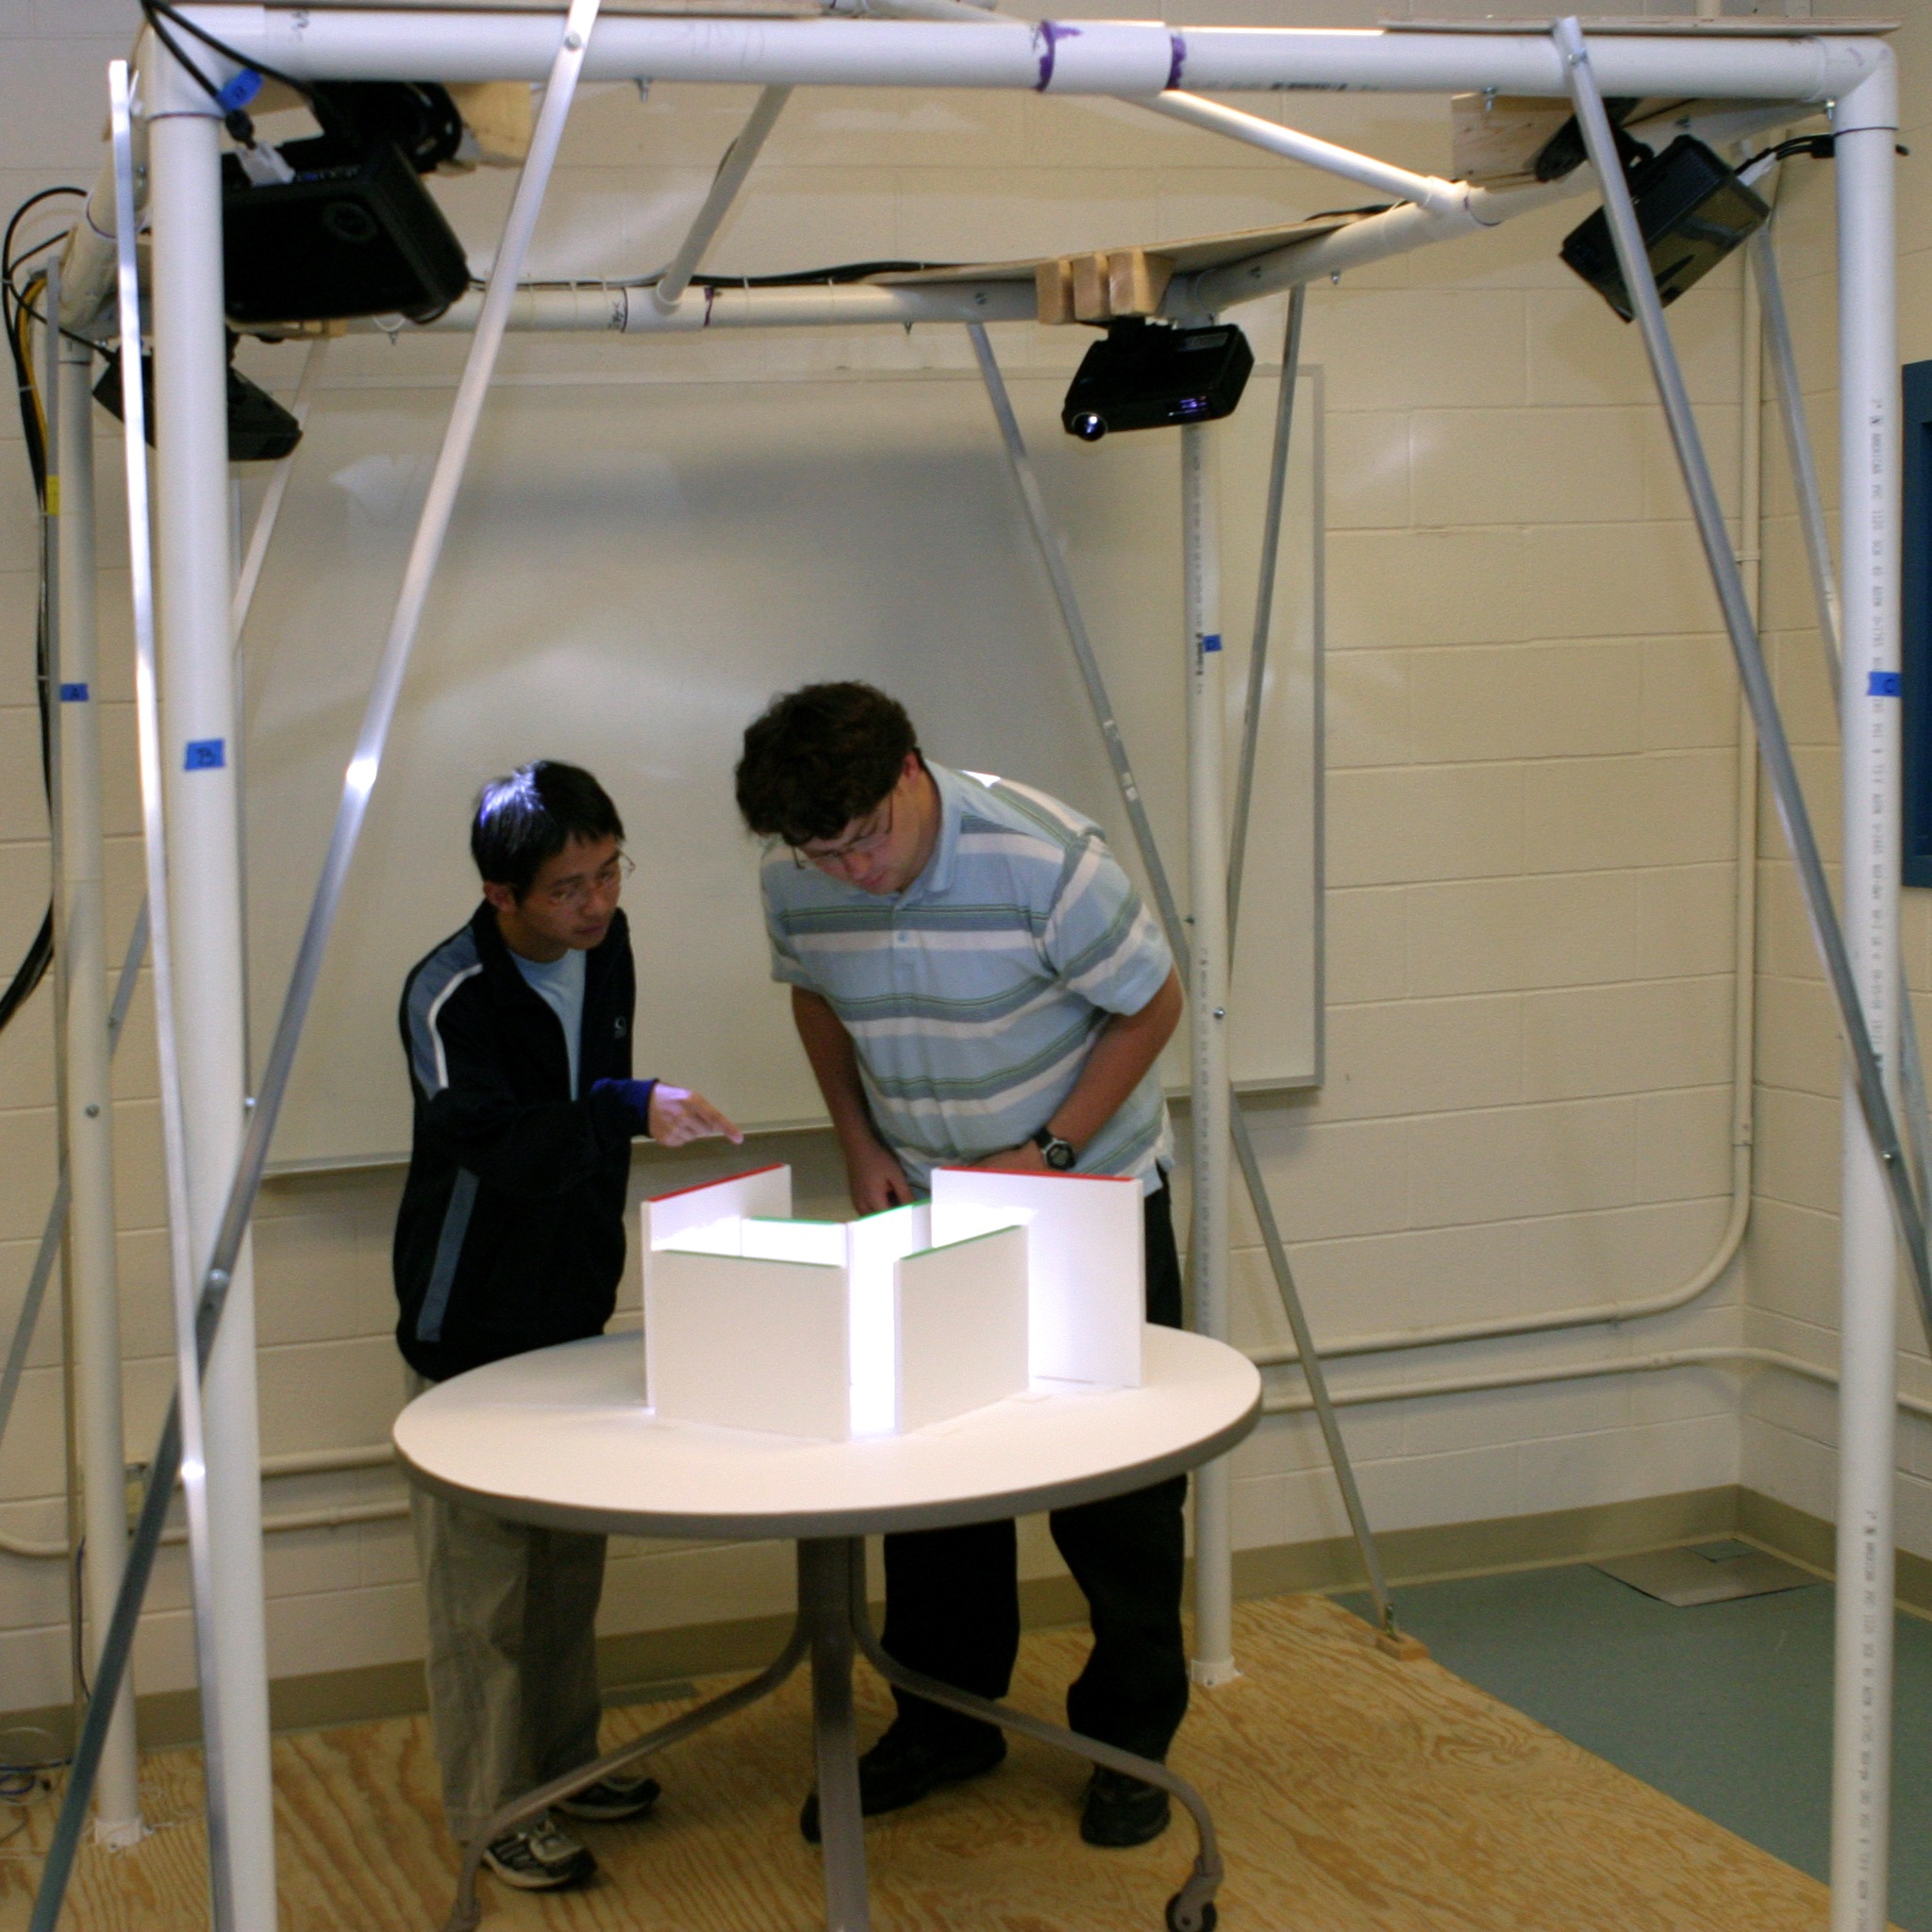
\includegraphics{aag2010_images/yu_stuetzle_contraption}}
\resizebox{!}{0.98in}{\includegraphics{aag2010_images/cshape_slr_model}}
\resizebox{!}{0.98in}{\includegraphics{aag2010_images/cshape_annotated}}
\resizebox{!}{0.98in}{\includegraphics{aag2010_images/remesher_cshape}}
\vspace{-0.2in}
\\
\begin{minipage}{0.98in}\textcolor[rgb]{1,1,1}{\hspace{-0.01in} {\bf a)}} \end{minipage}
\begin{minipage}{1.30in}\textcolor[rgb]{0,0,0}{\hspace{-0.01in} {\bf b)}} \end{minipage}
\begin{minipage}{0.98in}\textcolor[rgb]{1,1,1}{\hspace{-0.01in} {\bf c)}} \end{minipage}
\begin{minipage}{1.20in}\textcolor[rgb]{0,0,0}{\hspace{-0.01in} {\bf d)}} \end{minipage}
\caption{In our physical architectural design environment a) users
  gather around a table and construct b) a small-scale mockup of a
  design from a collection of wall elements and marker tokens.  A
  camera above the table c) captures the layout of elements on the
  table.  Our sketch interpretation algorithm processes these elements
  to construct a consistent and watertight triangular mesh of the
  implied architectural design (ceiling removed for visualization). }
\label{figure:virtual_heliodon}
\end{figure}

%%%%%%%%%%%%%%%%%%%%%%%%%%%%%%%%%%%%%%%%%%%%%%%%%%%%%%%%%%%%%%%%%%%%%%%%
%\subsection{Contributions}

%In this paper we present the following contributions:

%\begin{itemize}

%\item The collection of several hundred physical architectural
%  sketches using our design environment.  Each design is annotated by
%  the original designer to indicate the intended interpretation of the
%  design.

%\item Re-interpretation of these designs by other humans to provide a
%  measure of the ambiguity present in these sketches.  The set of
%  human interpretations is compared to the algorithm's output for
%  validation.

%\end{itemize}

%\subsection{Overview}

%We summarize several important areas of related work in
%Section~\ref{section:related_work}.  In
%Section~\ref{section:sketch_interpretation} we present our sketch
%interpretation algorithm, which was developed with extensive user testing
%and feedback from both architects and non-architects.  In
%Section~\ref{section:user_study} we present the results of two formal user
%studies that we conducted to gather a large set of example designs and
%validate our sketch interpretation approach.

\begin{comment}
%%%%%%%%%%%%%%%%%%%%%%%%%%%%%%%%%%%%%%%%%%%%%%%%%%%%%%%%%%%%%%%%%%%%%%%%
\section{Related Work}

\label{section:related_work}

Our project draws from research in a wide variety of areas including:
sketching interfaces, sketch recognition, human perception, and
computational models of gestalt and saliency.  In the sections below
we provide a brief overview of prior art in these fields and existing
software for architectural design.

\subsection{Modeling Interfaces for Architectural Design}

Many existing computer software packages tackle the challenge of
constructing 3D architectural geometry.  Initially these packages
focused almost exclusively on creating models with high geometric
precision, requiring a significant investment of time and only limited
support for editing a completed model.  Unfortunately, because
focusing on precision too early in the design process can stifle
creativity~\cite{LAWSON}, these tools are generally used only in the
later stages of design.  

The requirements for 3D models in architecture vary tremendously
depending on the intended use of the model.  Photorealistic renderings
require high polygon count geometry and accurate normals and
materials.  In contrast, many simulations (e.g., acoustic, passive
ventilation, heating/cooling, structural analysis) require a
consistent and watertight geometric model for accurate calculations
and often perform most efficiently with a simplified model constructed
especially for that analysis~\cite{ecotect}.  

More recently, software tools have become more amenable to the fast-paced,
quick sketching of the early stages of design~\cite{sketchup}, including
explorations of pen-based user interfaces for 3D
modeling~\cite{Zeleznik:1996:SAI,teddy,And02correlation-basedreconstruction}.
A limited construction interface (axis-aligned elements on a floor plan
grid) can help ensure the construction of architectural environments that
are appropriate for use in virtual reality walkthroughs~\cite{mackie}.  New
drawing user interfaces and systems have been demonstrated that allow
architects to leverage their pen and paper skills when interacting with the
new media interface of the computer.  Using projective geometry, freehand
architectural sketches can be re-projected or warped to simulate novel
viewpoints and an immersive experience~\cite{tolba}.  The Mental Canvas
system allows designers to arrange 2D sketches on arbitrary planes in 3D,
constructing an effective representation of complex architectural
spaces~\cite{mental_canvas}.




%-----------------
\subsection{\bf Sketch Recognition}

Sketch recognition systems are typically custom-developed for each
application (e.g., recognizing hand drawn UML
diagrams~\cite{UML_diagrams}) and leverage domain-specific knowledge
to improve accuracy.  General-purpose toolkits and languages for
sketch recognition of diagram components can ease the development of
these programs~\cite{ladder}.  

Well-designed sketching user interfaces minimize the number of
times the user is prompted for additional information or design
annotation, which interrupts workflow and concentration.  Strategies
for continuous and incremental recognition of drawings as they develop
have been demonstrated~\cite{Alvarado01resolvingambiguities}.  It is
important to maintain an estimate of the confidence in the
intermediate interpretations, which improves the accuracy of the final
interpretation.
%sketch interpretation in real time, but with
%limited interruptions of the user to ask if the interpretation is
%correct.  incremental interpretation, interpretation revision in the
%presence of new sketch data
An ongoing challenge in sketch recognition is the grouping of multiple
individual strokes that form a single logical unit.  The drawing
sequence for individual strokes and other meta-data available from
tablet displays~\cite{wacom} can be used as evidence when tackling
this problem~\cite{gross_1994}.  Another challenge in sketch
recognition comes from touch-up or continuation strokes the user might
make to complete a drawing~\cite{paulson_phdthesis}.  These strokes
are disconnected from or overlap other strokes but are intended to be
recognized as a single object.  Spatially close strokes (often defined
as the distance between two endpoints being less than 10\% of their
average length) can be merged; however this greedy approach, while
fast enough for interactive sketching, is not optimal.
%Overtraced strokes are still challenging to detect and
%recognize and accuracy drops with complex shapes.  A hierarchical
%analysis of subshapes has potential.

%Principles of sketch recognition require understanding of the

%* confidence level reflects sketch recognition accuracy

\subsection{\bf Sketch Recognition for Architectural Drawings}

The precision, consistency, and standardization of architectural CAD
drawings make this domain amenable to automatic processing algorithms,
and an impressive collection of automated sketch recognition programs
have been developed for architectural
drawings~\cite{Ah-soon97variationson,architectural_symbol_recognition,kulikov_mastersthesis,Lu_electronic_architectural_drawings}.
The motivation behind many of these tools is the digitization and
automated reconstruction of 3D building geometry from older
construction documents.  These methods have also been demonstrated for
hand-drawn architectural designs that closely follow the diagrammatic
conventions of CAD
drawings~\cite{aoki_hand_sketched_floor_plans,llados_hough}. For
example, the VR Sketchpad project automatically interprets a 2D
floorplan sketch including furniture layout to create a 3D VRML model
that can be used for walkthroughs~\cite{vrsketchpad}.  Freehand
sketching can be used to interact with digital
models~\cite{Gross00drawingon} and preliminary work was done to
classify interior and exterior walls in quick floorplan
sketches~\cite{archiassist}.

Koutamanis and Mitossi describe three levels of automated recognition
of architectural floor plans: recognition of geometric elements,
recognition of building elements, and recognition of spatial
articulation \cite{Koutamanis_computer_vision}.  They argue that the
third category is the most advanced: identifying solid mass versus
space within the design.  Our aim in this work is to specifically
address this challenge for freeform architectural sketches using a
tangible interface.
%Koutamanis discusses strategies to represent uncertainty in design
%within digital models~\cite{koutamanis_fuzzy}.  


%----------------------------
\subsection{Gestalt Theory and Sketch Interpretation}

Gestalt psychology, the laws of perceptual organization, and
Pragnanz~\cite{koffka,kanizsa} describe how humans perceive and
interpret incomplete diagrams or other modes of partial stimuli.  The
fundamental phenomena of closure, proximity, symmetry, and continuity
can be explained by low level human vision processing.  Gestalt theory
describes why our interpretation of an incomplete or ambiguous diagram
tends toward simpler forms, avoiding complexity.  The rich vocabulary
of pen and paper sketching in architectural design draws on the
gestalt principles of collinearity, parallelism, continuation, and
completion~\cite{koutamanis_sketch_recognition}.  Our algorithm for
automated interpretation of architectural sketches follows and
implements these principles.  Our user studies on human interpretation
of architectural sketches provides validation to our proposed use of
these concepts in recognition and analysis of architectural designs.

Research in computer vision has developed algorithms for image
processing using computational models of gestalt.  Attributes which
define the form, i.e., thickness of a line, convexity, and
parallelism, can be referred to as {\em gestalts}~\cite{desol02}.
Computational gestalt research focuses on determining thresholds that
indicate a pattern is significant.  In other words, this work involves
detecting and studying patterns and analyzing how likely those
patterns would be to occur in the image randomly~\cite{desol02}.
%While
%we are not explicitly using computational gestalt in our algorithm we
%do use something very similar to it in order to interpret the designs.
%We have to do a similar analysis to computational gestalt to decide if
%walls are meant to be collinear.

Similarly, saliency is a measure of how much an area stands out in
comparison to the areas around it. 
%
A {\em saliency map}~\cite{koch85} combines different stimuli
(movement, color, etc.) and the relative conspicuity to quantify changes 
in these characteristics.
%Detecting salient areas of an
%image is an important in Computer Vision.  
Itti, Koch and Niebur designed a computational visual attention model
based on the primate visual system to estimate the saliency map and
identify which areas of the scene are most likely to contain useful
information and should be analyzed in more detail~\cite{itti98}.
%
%~\cite{siag} 
%Saliency to aid in their robot localization system.
%Along with finding the "gist" of the scene, salient regions are used
%in a Monte-Carlo method to deduce it's location.
%Research continues to be
%done using Saliency such as Decarlo who created a program that
%transforms a photo into a line drawing by tracking a user's eye
%movements and keeping the most detail where the user focuses
%~\cite{decarlo02}. 
%Research has also been continuing on finding faster
%ways to obtain saliency maps such as using GPU's ~\cite{long06}.


%%%%%%%%%%%%%%%%%%%%%%%%%%%%%%%%%%%%%%%%%%%%%%%%%%%%%%%%%%%%%%%%%%%%%%%%
\section{Sketch Interpretation Algorithm}

\label{section:sketch_interpretation}

In our physical sketching environment, the user selects from the provided
collection of physical props and quickly assembles the chosen pieces on the
table.  Thus, the arrangement of elements truly forms a rough, approximate
sketch.  The selected wall pieces are likely too long or too short,
yielding overlaps or gaps with adjacent walls.  Similarly, the limited
palette of curved components may not have the desired curvature and thus
tangential connections are imprecise.  Furthermore, the approximate
assembly manner means that components intended to be parallel or meet at
crisp $90\,^{\circ}$ angles will include some unavoidable imprecision.  The
challenge is to sift through the available information to deduce and
construct the clean and complete design as it was conceived in the
architect's mind.

In the following sections we present the key steps of our sketch
interpretation algorithm: image pre-processing, detecting parallel,
perpendicular, and collinear elements, linking elements into chains,
constructing an arrangement of polygonal cells, estimating spatial
enclosure, assigning interior/exterior zones, managing details, and
post-processing the floorplan geometry to make a 3D model.

%------------------------------------------------
\subsection{Image Pre-Processing}

A camera mounted above the table captures the details of the physical
sketch.  A controlled lighting environment and carefully chosen color-coded
labels on the physical elements allow this geometry to be robustly
detected using standard image processing techniques, which are described in
detail in our earlier publications~\cite{virtual_heliodon,tvcg2009}.

The input to our sketch interpretation algorithm is the 2D projection
of each detected wall module onto the table surface, labeled with the
element height.  The flat walls are rectangles and include any
associated windows as inscribed rectangles.  The circular arc curved
walls are specified by a center, the inner and outer radii, and the
start and end angles of the arc.  An example of this input is shown in
Figure~\ref{figure:colinearity}a.


%------------------------------------------------
\subsection{Intended Parallel, Perpendicular, and Collinear Elements}
\end{comment}
\begin{figure}[t]
\resizebox{0.74in}{0.74in}{\includegraphics{aag2010_images/colinearity_tolerance/20091028_00636_2D_walls}}
\resizebox{0.74in}{0.74in}{\includegraphics{aag2010_images/colinearity_tolerance/20091028_annotated_00636}}
\resizebox{0.74in}{0.74in}{\includegraphics{aag2010_images/colinearity_tolerance/20091028_00636_interp_026}}
\resizebox{0.74in}{0.74in}{\includegraphics{aag2010_images/colinearity_tolerance/20091028_00636_interp_033}}
\resizebox{0.74in}{0.74in}{\includegraphics{aag2010_images/colinearity_tolerance/20091028_00636_interp_036}}
\resizebox{0.74in}{0.74in}{\includegraphics{aag2010_images/colinearity_tolerance/20091028_00636_interp_075}}
%\resizebox{0.63in}{0.63in}{\includegraphics{aag2010_images/colinearity_tolerance/20091028_00636_floorplan}}
\vspace{-0.36in}
\\
\begin{minipage}{0.74in}\textcolor[rgb]{0,0,0}{\hspace{-0.01in} { a)}} \end{minipage}
\begin{minipage}{0.74in}\textcolor[rgb]{0,0,0}{\hspace{-0.01in} { b)}} \end{minipage}
\begin{minipage}{0.74in}\textcolor[rgb]{0,0,0}{\hspace{-0.01in} { c)}} \end{minipage}
\begin{minipage}{0.74in}\textcolor[rgb]{0,0,0}{\hspace{-0.01in} { d)}} \end{minipage}
\begin{minipage}{0.74in}\textcolor[rgb]{0,0,0}{\hspace{-0.01in} { e)}} \end{minipage}
\begin{minipage}{0.74in}\textcolor[rgb]{0,0,0}{\hspace{-0.01in} { f)}} \end{minipage}
\caption{Intended collinearity can be ambiguous: a) detected primitives, b)
  annotation by the original designer, and c-f) annotation by other users.}
\label{figure:colinearity}
\end{figure}
 
\begin{comment}
For practical construction and space efficiency reasons, most
real-world architecture involves parallel walls and sharp
$90\,^{\circ}$ corners.  Even within high-profile showpiece
architecture, spaces are typically arranged into regular patterns and
placed on a grid, sometimes with secondary grids that are offset
and/or rotated.  Many (but not all) designs created by participants
using our tangible sketching interface follow these conventions and we
can automatically detect the implied grid(s).

First, we cluster the flat walls into groups that are nearly parallel
and {\em snap} all walls in each group to their weighted average
direction.  Similarly, we compare the wall groups to each other and
those that are approximately perpendicular are snapped to be
orthogonal.  We found that an angle tolerance of $5\,^{\circ}$ was an
appropriate threshold across all of our collected design data.  This
tolerance was effective at cleaning up placement imprecision inherent
in the physical sketching environment, yet was not large enough to
introduce artifacts in the more freeform designs that eschewed
parallelism and right angles.

In addition to the angle tolerance, it is necessary to identify flat
walls that are approximately collinear.  However, selecting a global
setting for this offset tolerance distance is somewhat more difficult.
We also saw variable tolerances for collinearity in human perception
when different users were asked to interpret the same design
(Figure~\ref{figure:colinearity}).  Some users perceived a slight line
break as an intended straight line, while others interpreted the break
as an architectural feature and possibly an entrance.  We found that
using a 1'' offset distance tolerance in our physical sketching
environment (equal to 1' in full-scale) was a good compromise for our
automatic collinearity detection and adjustment, but the user may need
control of this threshold for some designs.


We have not yet finished implementation of similar clustering and
adjustment methods for circular arcs.  The implementation is
straightforward and will require determination of appropriate
tolerances and smoothing procedures for several cases: multiple arcs
placed to sketch a circle or ellipse (e.g.,
Figure~\ref{figure:colinearity}), two arcs that form an inflection
point, and adjustment of the tangent and/or curvature when a circular
arc leads into a flat, straight wall.

%------------------------------------------------
\subsection{Linking Walls to Form Continuous Chains}

Following the gestalt principle of continuity we not only snap nearly
collinear elements to a common line, but we also form explicit
connections between elements with similar tangents (straight to
straight, straight to curved, or curved to curved).  Two or more
elements can be connected into a {\em chain} that is traced through
the working plane, separating space into two regions.  Our angular and
offset distance tolerances for establishing a connection between two
elements is less strict than the parallel and collinear thresholds
described in the previous section, allowing the establishment of
longer freeform chains.  Examples of these chains are shown in
Figure~\ref{figure:cells}c.

Our algorithm for establishing the chains is as follows.  For each
endpoint of each wall element we search all other walls for the best
matching connection tangent.  If a pairwise connection is mutual
(element A selects element B as the best match for tangent direction
and offset distance and element B also selects element A as the best
match), then the connection is established.  If no connection is made
for a wall endpoint, then that end of the wall chain is simply
extended to infinity following the tangent of the wall at that
endpoint.  When a wall chain connects curved arcs, the chain may form
a U turn (Figure~\ref{figure:cells} second row), a closed loop
(Figure~\ref{figure:cells} third row), or other interesting shapes.
\end{comment}
\begin{figure}[t]
\resizebox{0.74in}{0.74in}{\includegraphics{aag2010_images/arrangement_examples/091_02766_2D_walls}}
\resizebox{0.74in}{0.74in}{\includegraphics{aag2010_images/arrangement_examples/091_annotated_02766}}
\resizebox{0.74in}{0.74in}{\includegraphics{aag2010_images/arrangement_examples/091_02766_wall_chains}}
\resizebox{0.74in}{0.74in}{\includegraphics{aag2010_images/arrangement_examples/091_02766_fingerprint}}
\resizebox{0.74in}{0.74in}{\includegraphics{aag2010_images/arrangement_examples/091_02766_enclosed_points}}
\resizebox{0.74in}{0.74in}{\includegraphics{aag2010_images/arrangement_examples/091_02766_floorplan}}\\
%
\resizebox{0.74in}{0.74in}{\includegraphics{aag2010_images/arrangement_examples/20091021_01108_2D_walls}}
\resizebox{0.74in}{0.74in}{\includegraphics{aag2010_images/arrangement_examples/20091021_annotated_01108}}
\resizebox{0.74in}{0.74in}{\includegraphics{aag2010_images/arrangement_examples/20091021_01108_wall_chains}}
\resizebox{0.74in}{0.74in}{\includegraphics{aag2010_images/arrangement_examples/20091021_01108_fingerprint}}
\resizebox{0.74in}{0.74in}{\includegraphics{aag2010_images/arrangement_examples/20091021_01108_enclosed_points}}
\resizebox{0.74in}{0.74in}{\includegraphics{aag2010_images/arrangement_examples/20091021_01108_floorplan}}\\
%
\resizebox{0.74in}{0.74in}{\includegraphics{aag2010_images/arrangement_examples/091_13151_2D_walls}}
\resizebox{0.74in}{0.74in}{\includegraphics{aag2010_images/arrangement_examples/091_annotated_13151}}
\resizebox{0.74in}{0.74in}{\includegraphics{aag2010_images/arrangement_examples/091_13151_wall_chains}}
\resizebox{0.74in}{0.74in}{\includegraphics{aag2010_images/arrangement_examples/091_13151_fingerprint}}
\resizebox{0.74in}{0.74in}{\includegraphics{aag2010_images/arrangement_examples/091_13151_enclosed_points}}
\resizebox{0.74in}{0.74in}{\includegraphics{aag2010_images/arrangement_examples/091_13151_floorplan}}\\
%
\resizebox{0.74in}{0.74in}{\includegraphics{aag2010_images/arrangement_examples/20091021a_00131_2D_walls}}
\resizebox{0.74in}{0.74in}{\includegraphics{aag2010_images/arrangement_examples/20091021a_annotated_00131}}
\resizebox{0.74in}{0.74in}{\includegraphics{aag2010_images/arrangement_examples/20091021a_00131_wall_chains}}
\resizebox{0.74in}{0.74in}{\includegraphics{aag2010_images/arrangement_examples/20091021a_00131_fingerprint}}
\resizebox{0.74in}{0.74in}{\includegraphics{aag2010_images/arrangement_examples/20091021a_00131_enclosed_points}}
\resizebox{0.74in}{0.74in}{\includegraphics{aag2010_images/arrangement_examples/20091021a_00131_floorplan}}
\\
\resizebox{0.74in}{0.74in}{\includegraphics{aag2010_images/graphcut_example/088_08661_2D_walls}}
\resizebox{0.74in}{0.74in}{\includegraphics{aag2010_images/graphcut_example/088_annotated_08661}}
\resizebox{0.74in}{0.74in}{\includegraphics{aag2010_images/graphcut_example/088_08661_wall_chains}}
\resizebox{0.74in}{0.74in}{\includegraphics{aag2010_images/graphcut_example/088_08661_fingerprint}}
\resizebox{0.74in}{0.74in}{\includegraphics{aag2010_images/graphcut_example/088_08661_enclosed_points}}
\resizebox{0.74in}{0.74in}{\includegraphics{aag2010_images/graphcut_example/088_08661_floorplan}}
\vspace{-0.35in}
\\
\begin{minipage}{0.74in}\textcolor[rgb]{0,0,0}{\hspace{-0.01in} { a)}} \end{minipage}
\begin{minipage}{0.74in}\textcolor[rgb]{0,0,0}{\hspace{-0.01in} { b)}} \end{minipage}
\begin{minipage}{0.74in}\textcolor[rgb]{0,0,0}{\hspace{-0.01in} { c)}} \end{minipage}
\begin{minipage}{0.74in}\textcolor[rgb]{0,0,0}{\hspace{-0.01in} { d)}} \end{minipage}
\begin{minipage}{0.74in}\textcolor[rgb]{0,0,0}{\hspace{-0.01in} { e)}} \end{minipage}
\begin{minipage}{0.74in}\textcolor[rgb]{0,0,0}{\hspace{-0.01in} { f)}} \end{minipage}
\caption{Dividing space into cells by extending tangents and connecting
  elements:  a) detected primitives, b) annotation by original designer,
  c) wall chains, d) zones defined by the wall chains, e) enclosure, and f)
  our automatic interpretation. }
\label{figure:cells}
\end{figure}
\begin{comment}
Defined spaces in architecture can be created by real and/or implied
boundaries.  Each wall chain divides the working plane into two
spaces, one on either ``side'' of the chain.  The set of all wall
chains in a model will divide space into many subspaces that can be
labeled by their sidedness, which is visualized in
Figure~\ref{figure:cells}d.  If a wall chain loops around and crosses
itself (Figure~\ref{figure:cells} fourth row, blue and yellow chains),
the loop portion of the chain is disconnected to define a new chain to
allow the unique labeling of all subspaces.  Note that if two wall
chains cross two or more times (which is possible if one or both
chains are non-linear), the resulting subspace organization may have
two disconnected spaces that have the same sidedness
(Figure~\ref{figure:cells} fifth row, blue and red cells).  We perform
a connected component analysis to identify this situation and define
separate subspaces.

%------------------------------------------------
\subsection{Arrangement of Cells and Enclosure}

The wall chains described in the previous section are used to cut the
working plane into a watertight planar convex polygonal mesh or
arrangement of cells, which is represented using a half-edge data
structure.  Each wall chain explicitly represents the wall thickness,
thus working plane polygons are constructed for both open space
(interiors and exteriors) as well as the are comprising the
construction thickness of real and implied walls.

For each cell in the arrangement, we calculate the {\em enclosure},
the probability that the cell is part of the building interior.  We
define the enclosure at a point as the lack of visibility to areas
outside of the design from that point.  We estimate this value by
tracing rays from the point to infinity in a dense sampling of
directions and record the fraction of all rays that intersect a wall
of the design.  We visualize enclosure over a dense point grid in
Figure~\ref{figure:cells}d.  Points with high enclosure (nearly all
rays intersect a wall in the design) are drawn light grey or white,
and points with low enclosure are dark grey.  We define the average
enclosure of the cell in the arrangement by averaging the enclosure at
many points within the cell.  Similarly, we can compute the average
and standard deviation of the point-based enclosure values for a
subspace.

For relatively simple designs, a carefully-selected global threshold
placed on the point/cell/subspace enclosure value can correctly
classify each subspace as interior or exterior.  However, as the gaps
between the walls increase or decrease the threshold value must be
adjusted accordingly (compare the first and third rows of
Figure~\ref{figure:cells}d).  Furthermore, if the model contains
concavities in the outer wall, nearby areas may be incorrectly marked
as interior spaces.  Beyond the challenge of selecting a threshold,
for more complex models a simplistic setting of a global threshold
will not successfully separate the building interior from exterior
(Figure~\ref{figure:nonconvex}).

One cause for incorrect interior/exterior division is high variance in
enclosure within a single subspace.  For example, consider the final row of
Figure~\ref{figure:cells}.  The sharp bends of the blue wall chain loop
through the design and interact with the other two wall chains to produce
one large subspace, colored cyan and green.  The enclosure values within
this subspace have high variance, indicating that it should not be treated
as a single space when identifying interior space.  For each subspace with
high enclosure variance, we solve a Minimum Cut graph problem to determine
an optimal segmentation of this subspace.  We build a dual graph from the
polygonal cells in this subspace.  Each polygonal cell in the arrangement
is a node in the graph.  If two cells share an edge in the arrangement, we
create an edge between the corresponding nodes in the graph.  The weight of
the edge is defined to be the length of the shared edge in the arrangement.
The source is defined to be the node whose corresponding cell has the
highest enclosure, and the sink is likewise defined to be the cell with the
lowest enclosure value.  Using a basic textbook implementation of the
Maximum Flow/Minimum Cut algorithm, we find a minimum length cut which
divides the zone into two subspaces that will have lower variance and
produce a more satisfactory interior/exterior segmentation of the design.
\end{comment}
\begin{figure}[t]

\resizebox{0.74in}{0.74in}{\includegraphics{aag2010_images/courtyard/20091014_annotated_03526}}
\resizebox{0.74in}{0.74in}{\includegraphics{aag2010_images/courtyard/20091014_03526_enclosed_points}}
\resizebox{0.74in}{0.74in}{\includegraphics{aag2010_images/courtyard/20091014_03526_floorplan}}
%
\resizebox{0.74in}{0.74in}{\includegraphics{aag2010_images/courtyard/040_annotated_07372}}
\resizebox{0.74in}{0.74in}{\includegraphics{aag2010_images/courtyard/040_07372_enclosed_points}}
\resizebox{0.74in}{0.74in}{\includegraphics{aag2010_images/courtyard/040_07372_floorplan}}
\\
\resizebox{0.74in}{0.74in}{\includegraphics{aag2010_images/courtyard/066_annotated_03260}}
\resizebox{0.74in}{0.74in}{\includegraphics{aag2010_images/courtyard/066_03260_enclosed_points}}
\resizebox{0.74in}{0.74in}{\includegraphics{aag2010_images/courtyard/066_03260_floorplan}}
%
\resizebox{0.74in}{0.74in}{\includegraphics{aag2010_images/courtyard/20091014_annotated_02020}}
\resizebox{0.74in}{0.74in}{\includegraphics{aag2010_images/courtyard/20091014_02020_enclosed_points}}
\resizebox{0.74in}{0.74in}{\includegraphics{aag2010_images/courtyard/20091014_02020_floorplan}}
\caption{Designs with non convex boundaries may not be accurately
  extracted with a simple threshold on the average point or cell
  enclosure.  By minimizing the lengths of unused wall and extra {\em
    inferred wall} necessary to enclose the interior zones we 
  correctly interpret these complex designs.}
\label{figure:nonconvex}
\end{figure}

\begin{comment}
%------------------------------------------------
\subsection{Assigning Interior and Exterior Zones}


After the wall chains have divided the working plane into a set of
zones, we need to label each zone as either an interior or exterior
space.  The average enclosure value for the zone can be used to make
an initial determination, but that strategy frequently yields
incorrect assignments for complex designs with non-convex boundaries
(e.g., Figure~\ref{figure:multiple_rooms}).  Furthermore, our method
for constructing wall chains that extend each element to infinity will
yield a division of space into zones far from the element's actual
position, which may not be intended.  When two neighboring zones are
assigned opposite labels, the wall or wall chain between the zone is
thus interpreted as an implied wall or boundary.  If the original wall
element is short and/or a significant distance from the implied
boundary, the resulting automatically-constructed floor plan may be
non intuitive and not match a human interpretation.  Therefore, we
must be careful to use an extended wall chain as evidence for a
boundary only in close proximity to the original wall.  Every
hypothesized or inferred wall separating interior and exterior space
should be checked against the evidence.
\end{comment}
\begin{figure}[t]
\resizebox{0.74in}{0.74in}{\includegraphics{aag2010_images/multiple_rooms_examples/20091028_00908_2D_walls}}
\resizebox{0.74in}{0.74in}{\includegraphics{aag2010_images/multiple_rooms_examples/20091028_annotated_00908}}
\resizebox{0.74in}{0.74in}{\includegraphics{aag2010_images/multiple_rooms_examples/20091028_00908_floorplan}}
%
\resizebox{0.74in}{0.74in}{\includegraphics{aag2010_images/multiple_rooms_examples/013_03253_2D_walls}}
\resizebox{0.74in}{0.74in}{\includegraphics{aag2010_images/multiple_rooms_examples/013_annotated_03253}}
\resizebox{0.74in}{0.74in}{\includegraphics{aag2010_images/multiple_rooms_examples/013_03253_floorplan}}
%
\resizebox{0.74in}{0.74in}{\includegraphics{aag2010_images/multiple_rooms_examples/013_01221_2D_walls}}
\resizebox{0.74in}{0.74in}{\includegraphics{aag2010_images/multiple_rooms_examples/013_annotated_01221}}
\resizebox{0.74in}{0.74in}{\includegraphics{aag2010_images/multiple_rooms_examples/013_01221_floorplan}}
%
\resizebox{0.74in}{0.74in}{\includegraphics{aag2010_images/multiple_rooms_examples/013_05156_2D_walls}}
\resizebox{0.74in}{0.74in}{\includegraphics{aag2010_images/multiple_rooms_examples/013_annotated_05156}}
\resizebox{0.74in}{0.74in}{\includegraphics{aag2010_images/multiple_rooms_examples/013_05156_floorplan}}
%
\vspace{-0.25in}
\caption{
Challenging examples of designs with multiple rooms.  The
  examples in the bottom row are somewhat ambiguous and have multiple
  reasonable interpretations for the passageways between rooms. 
\vspace{-0.1in}
 }
\label{figure:multiple_rooms}
\end{figure}
\begin{comment}

In solving this problem, we follow the Gestalt principles of closure
and simplicity.  We search for a closed form that is simple, uses most
or all of the detected wall elements, and requires little length of
additional inferred exterior wall to fill gaps between the original
wall primitives of the sketch.  We solve this optimization problem in
a brute force manner by considering as interior space all subsets of
the zones with enclosure values above a reasonable threshold and
select the zone assignment that minimizes the sum of all unused walls
and all inferred walls.  An unused wall is defined as a detected
element that has exterior zone on both sides.  Note that wall elements
may be partially used and the unused wall penalty is accordingly
prorated.  Similarly, an inferred wall is a portion of wall chain that
is not represented in the sketch by a physical wall, but has exterior
zone on one side and interior zone on the other.  In the floor plan
results diagrams used throughout this paper, real walls are drawn in
black, interior zones are drawn in medium grey, exterior zones are
white and inferred walls are drawn in dark red for visualization
purposes.


Some of the collected designs contain an interior space that might
have been conceived as an open courtyard rather than a room with no
exterior walls (Figure~\ref{figure:courtyards}).  This distinction can
be important for architectural simulations such as daylighting design
or passive ventilation --- whether the finished design includes a roof
over this fully interior room will impact the simulated performance
results.  To resolve this ambiguity, we are considering user interface
options for allowing the designer to indicate which of these two
perfectly reasonable scenarios he/she intended.  Importantly, we want
maintain our minimalist interface and follow the most appropriate
default interpretation.

%------------------------------------------------
\subsection {Detecting Inferred Interior Walls and Trimming Unused Walls}

\begin{figure}[t]
\resizebox{0.74in}{0.74in}{\includegraphics{aag2010_images/courtyard/20091028_00772_interp_036}}
\resizebox{0.74in}{0.74in}{\includegraphics{aag2010_images/courtyard/20091028_00772_floorplan}}
%
\resizebox{0.74in}{0.74in}{\includegraphics{aag2010_images/courtyard/060_12354_interp_018}}
\resizebox{0.74in}{0.74in}{\includegraphics{aag2010_images/courtyard/060_12354_floorplan}}
%
\resizebox{0.74in}{0.74in}{\includegraphics{aag2010_images/courtyard/066_annotated_05996}}
\resizebox{0.74in}{0.74in}{\includegraphics{aag2010_images/courtyard/066_05996_floorplan}}
\caption{If the design contains a interior room with no exterior
  walls, this space may be intended as a courtyard space, uncovered by
  a roof. The system will require extra information from the designer
  if the default interpretation does not match his/her intentions. }
\label{figure:courtyards}
\end{figure}


Once the core interior/exterior spaces of the design have been
determined and the true exterior and inferred exterior walls have been
identified, the system performs several small cleanup steps to improve
the quality of the final model and ensure that the extracted 3D
geometry is manifold.
%
When two wall chains that each define a portion of the boundary
between interior and exterior cross, the quadrilateral zone defined by
the thickness of each chain at the crossing should also be labeled as
a wall to create proper interior and exterior corners.

Some designs incorporate interior partition walls that are meant to
separate the interior into smaller rooms.  Due to the physical
sketching environment, generally these walls are a bit short and leave
small gaps where they should meet other interior or exterior walls.
However, not all gaps should be closed.  Standard doorways in
architecture are generally a minimum of 2'6'' wide, so if the gap is
less than 2'' wide, we assume this was intended to be a solid wall and
we close the gap by labeling the corresponding wall chain polygons as
inferred walls.  We found that this tolerance provided a reasonable
match to the designer's annotation of his/her intentions for the full
range of example designs.
%
Similarly, when the physical wall modules are slightly too long and
protrude from the middle of an inferred boundary or corner, we should
clip back this geometry to create a more polished design.  We propose
a tolerance of 1'' (corresponding to 1' in full scale) for this
trimming.  We note that it is important to not completely remove from
the design all walls that are ``unused'' (not positioned on the
exterior/interior boundary of the model or used as interior
partitions).  In many cases these extra exterior walls serve specific
architectural functions including privacy screens, shading, acoustic
dampening, and wind control.

Finally, we propose an initial strategy for labeling the primary
entrance to a design, and augmenting the floorplan and 3D model with
this information.  Note that not all designs have a clear entrance,
but many of our user study participants left specific openings within
the outer boundary of their shape.  Simply detecting the longest
section of inferred exterior boundary (and greater than a minimum
tolerance of approximately 4'') as the primary entrance will correctly
label this feature in most of the designs.  One notable example that
breaks this rule is shown in the bottom row of
Figure~\ref{figure:domain_specific}.  Annotations made by other user
study participants match the intention of the original designer: the
obvious entrance is through an elaborate portico, rather than through
one of the large gaping holes in the ``back'' of the design.  This
sketch interpretation task will benefit from domain-specific knowledge
of common architectural forms.
\end{comment}
\begin{figure}[t]
\resizebox{0.74in}{0.74in}{\includegraphics{aag2010_images/domain_specific_examples/20091028a_annotated_00762}}
\resizebox{0.74in}{0.74in}{\includegraphics{aag2010_images/domain_specific_examples/20091028a_00762_interp_026}}
\resizebox{0.74in}{0.74in}{\includegraphics{aag2010_images/domain_specific_examples/20091028a_00762_interp_029}}
\resizebox{0.74in}{0.74in}{\includegraphics{aag2010_images/domain_specific_examples/20091028a_00762_interp_036}}
\resizebox{0.74in}{0.74in}{\includegraphics{aag2010_images/domain_specific_examples/20091028a_00762_interp_080}}
\resizebox{0.74in}{0.74in}{\includegraphics{aag2010_images/domain_specific_examples/20091028a_00762_floorplan}}
\\
\resizebox{0.74in}{0.74in}{\includegraphics{aag2010_images/domain_specific_examples/092-2_annotated_05027}}
%\resizebox{0.74in}{0.74in}{\includegraphics{aag2010_images/domain_specific_examples/092-2_05027_interp_017}}
\resizebox{0.74in}{0.74in}{\includegraphics{aag2010_images/domain_specific_examples/092-2_05027_interp_018}}
\resizebox{0.74in}{0.74in}{\includegraphics{aag2010_images/domain_specific_examples/092-2_05027_interp_026}}
\resizebox{0.74in}{0.74in}{\includegraphics{aag2010_images/domain_specific_examples/092-2_05027_interp_032}}
%\resizebox{0.74in}{0.74in}{\includegraphics{aag2010_images/domain_specific_examples/092-2_05027_interp_049}}
\resizebox{0.74in}{0.74in}{\includegraphics{aag2010_images/domain_specific_examples/092-2_05027_interp_067}}
\resizebox{0.74in}{0.74in}{\includegraphics{aag2010_images/domain_specific_examples/092-2_05027_floorplan}}
\vspace{-0.35in}
\\
\begin{minipage}{0.74in}\textcolor[rgb]{0,0,0}{\hspace{-0.01in} { a)}} \end{minipage}
\begin{minipage}{0.74in}\textcolor[rgb]{0,0,0}{\hspace{-0.01in} { b)}} \end{minipage}
\begin{minipage}{0.74in}\textcolor[rgb]{0,0,0}{\hspace{-0.01in} { c)}} \end{minipage}
\begin{minipage}{0.74in}\textcolor[rgb]{0,0,0}{\hspace{-0.01in} { d)}} \end{minipage}
\begin{minipage}{0.74in}\textcolor[rgb]{0,0,0}{\hspace{-0.01in} { e)}} \end{minipage}
\begin{minipage}{0.74in}\textcolor[rgb]{0,0,0}{\hspace{-0.01in} { f)}} \end{minipage}
\caption{Domain-specific knowledge may be necessary to correctly
  interpret sketches that hint at common architectural forms, such as
  the cruciform used in church floor plans (top row) or to recognize
  an entrance portico (bottom row).  Despite the potential for
  ambiguity, b-e) most users' interpretations matched a) the original
  designer's intention.  Our automatic sketch interpretation results
  are shown in f). }
\label{figure:domain_specific}
\end{figure}
\begin{comment}
%------------------------------------------------
\subsection{Post-Processing: Constructing a Watertight Triangle Mesh}

At the end of our sketch interpretation algorithm, we have a precise,
manifold, polygonal representation of the working plane.  Each
polygonal cell has well defined neighboring cells (no 'T' junctions)
and has been assigned one of several labels: {\em solid wall}, {\em
  window within a wall}, {\em interior space}, or {\em exterior
  space}.  This representation can be extruded and exported as a
consistent mesh following the necessary CAD conventions for
architectural rendering or performance simulation software.  For
example, we can construct a watertight mesh appropriate for a
radiosity simulation of interior illumination as follows.  Each
interior cell is exported as two polygons, one floor plane polygon
with normal pointing 'up' and one ceiling polygon with normal pointing
'down'.  For every edge between an interior cell and a wall or
exterior cell, we create a wall polygon stretching from the floor to
the ceiling with normal pointing toward the interior cell.  When an
interior cell touches a window cell, the exported wall polygon is
split vertically and assigned different materials as appropriate.


%%%%%%%%%%%%%%%%%%%%%%%%%%%%%%%%%%%%%%%%%%%%%%%%%%%%%%%%%%%%%%%%%%%%%%%%
%%%%%%%%%%%%%%%%%%%%%%%%%%%%%%%%%%%%%%%%%%%%%%%%%%%%%%%%%%%%%%%%%%%%%%%%
\end{comment}
\subsection{Validation of Physical Sketch Interpretation Environment}

\label{section:user_study}

To validate our algorithm for sketch interpretation, we ran two user
studies, one focusing on our physical sketching environment and the
second on sketch interpretation.  We recruited participants with a
variety of backgrounds including architecture, visual arts, and
computer science.

\subsection{Design Collection Study}

The purpose of the first user study was to sample the range of
architectural designs that could be constructed in our physical
sketching environment and to evaluate the potential for its use in the
early stages of architectural design.  The design task was open-ended
and after a brief overview of the tangible interface, participants
were instructed to use the wall and window primitives to create
between 10 and 20 different designs.

%free to design whatever
%space (room or building) they wanted,
%but we constrained them to using four types of primitives:
%straight walls, curved walls, columns and window markers.  
%Each
%participant was asked to create between 10 and 20 different
%intermediate or final designs and was allowed to finish sooner if they
%so desired.

After each participant completed the design stage, we prepared a
single-page annotation form for each of his/her designs.  The form
contained two parts: {\em designer annotation} and {\em evaluation of
  automated sketch interpretation algorithm}.  The form was folded in
half so that only the annotation section was visible and the
participant was instructed to first complete the annotation for all
designs before unfolding the paper to see the output from our
automated sketch interpretation algorithm.  Thus, the participants
were not influenced by the output of our program in either the design
or annotation stages.

%
%handed the users a stack of print-outs which were folded in
%half, only revealing the top half.  
%They were told to keep the paper
%folded until instructed otherwise; the second half was concealed
%because an unfair bias would be introduced if users were able to see
%the algorithm's interpretation before annotating their own design.
%

The annotation portion of the form presented two large images: the
overhead photograph of the physical sketching environment (for
reference) and a 2D rendering of the detected wall geometry (to be
used for annotation).  The participant was instructed to use a green
highlighter to draw the complete intended wall geometry on the
detected geometry rendering. The pink, orange, and yellow highlighters
were used to shade interior spaces.  Optionally, he/she could use a
blue arrow to indicate an entrance or to sketch the circulation within
the design.  As guidance, users were provided with three example
designs annotated in this manner.

The evaluation portion of the paper contained our automatically
generated floor plan of the design.  The users were asked to evaluate
the quality of the automatic interpretation of each design, whether
it matched the design intention, was an acceptable alternate
interpretation, or was incorrect.
%given the options of choosing whether our algorithm
%detected the interior and exterior partitioning of the design well,
%whether they thought that it did poorly and with an improved algorithm
%should be able to do better, or if they thought that the design was
%too hard for a computer to interpret.  
Additionally, we encouraged them to mark or comment on which parts of
the design were most challenging for the automated system to
interpret.  After completing the evaluation of all designs, the users
filled out a short post-study questionnaire.

%\subsection{Participant Background Profile}

%Each participant filled out a short survey on the
%We For each participant Three types of participants were used in our study: architecture
%students, visual art students and miscellaneous students.
%Architecture students were chosen because they are the target audience
%for our tool, visual art students were chosen because of their
%extensive design background and miscellaneous students were used
%because they were available when needed.  

Each participant used our physical sketching environment for approximately
20 minutes and created 3-26 designs.  Some users created just
a few highly detailed designs, while others created many rough sketches or
a series of variations that evolved from a base sketch.  In total we
collected 329 designs from 30 participants in the first user study.
Fifteen of those participants (responsible for 154 of the designs) were
architecture students, most with at least three years of formal
architectural education and professional experience through
internships. 
Of the other participants, eight were visual arts students (83 designs) and
the remaining seven (92 designs) had no formal training in architecture or
art.  A broad selection of these designs are presented in
Figure~\ref{figure:lotsofdesigns}.


\subsection{Re-Interpretation Study to Quantify Design Ambiguities}

For the second study, we wanted to understand any discrepancies
between our algorithm's interpretation and the original designer's
intentions.  We wanted to investigate whether the differences were due
to a flawed automatic interpretation strategy or the result of
ambiguous physical sketches (Figure~\ref{figure:ambiguous}).  In order
to quantify the ambiguity of a particular design, in our second user
study we asked the participants to annotate a selection of interesting
sketches made by other users.  All participants for the second study
first performed the tasks of the first study (if they were not already
subjects in that study) and thus all were familiar with the sketching
environment and annotation instructions.


\begin{figure}[t]
\resizebox{0.74in}{0.74in}{\includegraphics{aag2010_images/ambiguous/039_annotated_05993}}
\resizebox{0.74in}{0.74in}{\includegraphics{aag2010_images/ambiguous/039_05993_interp_026}}
\resizebox{0.74in}{0.74in}{\includegraphics{aag2010_images/ambiguous/039_05993_interp_033}}
\resizebox{0.74in}{0.74in}{\includegraphics{aag2010_images/ambiguous/039_05993_interp_080}}
\resizebox{0.74in}{0.74in}{\includegraphics{aag2010_images/ambiguous/039_05993_interp_087}}
\resizebox{0.74in}{0.74in}{\includegraphics{aag2010_images/ambiguous/039_05993_floorplan}}\\
%
\resizebox{0.74in}{0.74in}{\includegraphics{aag2010_images/ambiguous/20091014_annotated_02500}}
\resizebox{0.74in}{0.74in}{\includegraphics{aag2010_images/ambiguous/20091014_02500_interp_018}}
\resizebox{0.74in}{0.74in}{\includegraphics{aag2010_images/ambiguous/20091014_02500_interp_026}}
\resizebox{0.74in}{0.74in}{\includegraphics{aag2010_images/ambiguous/20091014_02500_interp_059}}
\resizebox{0.74in}{0.74in}{\includegraphics{aag2010_images/ambiguous/20091014_02500_interp_087}}
\resizebox{0.74in}{0.74in}{\includegraphics{aag2010_images/ambiguous/20091014_02500_floorplan}}\\
%
\resizebox{0.74in}{0.74in}{\includegraphics{aag2010_images/ambiguous/20091021_annotated_00946}}
\resizebox{0.74in}{0.74in}{\includegraphics{aag2010_images/ambiguous/20091021_00946_interp_017}}
\resizebox{0.74in}{0.74in}{\includegraphics{aag2010_images/ambiguous/20091021_00946_interp_018}}
\resizebox{0.74in}{0.74in}{\includegraphics{aag2010_images/ambiguous/20091021_00946_interp_036}}
\resizebox{0.74in}{0.74in}{\includegraphics{aag2010_images/ambiguous/20091021_00946_interp_090}}
\resizebox{0.74in}{0.74in}{\includegraphics{aag2010_images/ambiguous/20091021_00946_floorplan}}\\
%
\resizebox{0.74in}{0.74in}{\includegraphics{aag2010_images/ambiguous/20091028b_annotated_00507}}
\resizebox{0.74in}{0.74in}{\includegraphics{aag2010_images/ambiguous/20091028b_00507_interp_062}}
\resizebox{0.74in}{0.74in}{\includegraphics{aag2010_images/ambiguous/20091028b_00507_interp_033}}
\resizebox{0.74in}{0.74in}{\includegraphics{aag2010_images/ambiguous/20091028b_00507_interp_067}}
\resizebox{0.74in}{0.74in}{\includegraphics{aag2010_images/ambiguous/20091028b_00507_interp_080}}
\resizebox{0.74in}{0.74in}{\includegraphics{aag2010_images/ambiguous/20091028b_00507_floorplan}}
\vspace{-0.35in}
\\
\begin{minipage}{0.74in}\textcolor[rgb]{0,0,0}{\hspace{-0.01in} { a)}} \end{minipage}
\begin{minipage}{0.74in}\textcolor[rgb]{0,0,0}{\hspace{-0.01in} { b)}} \end{minipage}
\begin{minipage}{0.74in}\textcolor[rgb]{0,0,0}{\hspace{-0.01in} { c)}} \end{minipage}
\begin{minipage}{0.74in}\textcolor[rgb]{0,0,0}{\hspace{-0.01in} { d)}} \end{minipage}
\begin{minipage}{0.74in}\textcolor[rgb]{0,0,0}{\hspace{-0.01in} { e)}} \end{minipage}
\begin{minipage}{0.74in}\textcolor[rgb]{0,0,0}{\hspace{-0.01in} { f)}} \end{minipage}
\caption{Some ambiguous designs: a) the original designer's
  annotation, b-e) annotation by other users, f) our automatic sketch
  interpretation results. }
\label{figure:ambiguous}
\end{figure}


All designs from the first study that our initial sketch
interpretation program struggled with were selected (omitting near
duplicates), as well as other designs that we thought were ambiguous,
complex, or interesting.  We also included a number of simpler
designs, which had a single reasonable interpretation, as controls.
In total, 114 of the 329 total designs from the first study were
selected.  60 of these designs were created by architecture students,
28 were made by visual arts students, and 26 were from students with
no formal training in architecture or visual arts.
%
%designs from the 370  One
%hundred fourteen particularly interesting designs of the 370 from the
%the first study were chosen to be reinterpreted.  
%


Each participant for the second study was presented with annotation
paperwork for a randomly ordered, randomly selected subset of these
designs.  The annotation form consisted of three parts: {\em
  annotation}, {\em comparison to the original designer's intention}, and
{\em evaluation of automatic interpretation}.  The forms were folded
to conceal the second and third parts.

As in the first study, the participants were asked to mark their
interpretation of each sketched design and shade the interior spaces.
After approximately 20 minutes each participant was asked
to proceed to the second part of the study and any designs he/she had
not yet annotated were collected.

Next, the participant was asked to unfold the paper (keeping the third part
concealed) and compare his/her interpretation of each design to the
original designer's intention, marking whether the interpretations matched
or how the designer's physical sketch was ambiguous or unclear.  Finally,
after all comparisons were made, the participant unfolded the third and
final part of the form and evaluated our computer algorithm for automated
sketch interpretation.
%  After our programs interpretation.  In
%addition to asking the users a series of qualitative questions, we
%also had the users compare their own interpretation to the original
%designers intentions and to the computers interpretation.


%Designs were chosen randomly from the 114 selected; order was
%randomized to remove bias and to prevent reinterpreters from following
%a designers evolution of designs (as intermediate designs were used in
%the study as well).  

%Participants for the second study were required to have already
%completed the sketch interpretation study as it was necessary for them
%to be familiar with the design and annotation process.  We asked them
%to reinterpret the designs (pictures of wall, window and column
%primitives) of designs from the sketch interpretation study. 

We collected a total of 346 new annotations from 15 participants (124
annotations were made by architecture students, 82 by visual arts
students, and 140 by other students).  Each of the 114 designs received
between 3-6 new annotations.

\subsection{Validation Results: Subjective Feedback}


The users' questionnaires revealed how excited they were about our
physical sketching environment.  A visual arts student said the system
was ``Very intuitive, very clear.  Felt like playing with blocks as a
kid, but each block had a meaning.  Seeing each design in 3-D helped
spike the creativity.''  Another visual arts student commented: ``I was
really impressed with the software--it did a great job mapping what I
wanted.''  A second year architecture student said of the system ``I
was very surprised by the accuracy of the program for the most part.
Despite some errors, the interior and exterior implied spaces were
read pretty well.''  Other users were surprised at particular failings
for rules we had not yet implemented.  ``The program filled in a void
that was meant to be exterior, especially since I had windows on the
exterior parts of these walls to make that distinction.''

We used direct feedback from architecture students in pilot studies as
well as general observations about the designs they created to improve
our sketching environment and automatic interpretation algorithm.
These improvements include: addition of curved walls and column
primitives, control over window placement, detection of disjoint
spaces and interior courtyards, and handling designs with large gaps
in the exterior wall (typically, an implied entrance).  We are
motivated to continue this avenue of work and tackle the challenges of
detection and labeling of the different subspaces within the
interior, predicting interesting circulation patterns, etc.

% Many of the comments from the
%first user study were used to improve the algorithm before the second
%user study.  
%The quantitative questions from the second section of the
%printouts did not provide useful feedback because each user understood
%the questions to mean something slightly different.  As a result,
%these statistics are not discussed in detail in this paper.

The results of our second study can best by summed up by one student.
Interpretation was ``Often challenging.  Many designs were unclear,
difficult to interpret.  Others were extremely clear and easy.''  Some
users were surprised by the variety and complexity of designs possible
in the system.  A visual arts student said ``I was surprised at the
designs that the other users came up with -- they seemed very complex
in some cases -- and the computer did a good job of interpreting
them.''

%In this study it was shown that the success with which the algorithm and
%humans interpret matched up well with the non-ambiguous cases.  
We found that for many of the designs that our algorithm struggled to
interpret, other humans also found the design to be ambiguous.
%Many of the designs that For most For designs where the
%algorithm misinterpreted the designer's intention, the human
%interpreters also either thought the design was ambiguous or came up
%with vastly different interpretations.
%92-2 5027 20091104a 669 and 992 
However, there were several notable examples where all humans
interpreted the design quite similarly to the original designer,
despite a lack of hard evidence for that shape within the sketch.
Figure~\ref{figure:domain_specific} presents a few of these examples,
where the humans are quite consistent in their interpretation of the
design.  We believe this may be due to domain-specific knowledge of
architectural forms that have not yet been explicitly encoded in our
sketch interpretation algorithm.
%
One architecture student noted for the example shown in the top row of
Figure~\ref{figure:domain_specific}: ``Humans recognize this because it
is a basic cruciform shape, but without more information, it may be
difficult for an algorithm to determine this.''


\subsection{Quantitative Sketch Interpretation Results}

\begin{table}[t]
\begin{center}
\begin{tabular}{c|rr|rr|rr|r}
           &  \multicolumn{2}{c|}{correct} & \multicolumn{2}{c|}{mostly correct}     & \multicolumn{2}{c|}{incorrect}          & total\\ \hline
clear      & \hspace{0.1in}155 & 78\% \hspace{0.1in} & \hspace{0.1in} 17 &  9\% \hspace{0.1in} & \hspace{0.1in} 26 & 13\% \hspace{0.1in} & 198\\
ambiguous  & \hspace{0.1in} 74 & 56\% \hspace{0.1in} & \hspace{0.1in} 35 & 27\% \hspace{0.1in} & \hspace{0.1in} 22 & 17\% \hspace{0.1in} & 131\\ \hline
total      & \hspace{0.1in}229 & 70\% \hspace{0.1in} & \hspace{0.1in} 52 & 15\% \hspace{0.1in} & \hspace{0.1in} 48 & 15\% \hspace{0.1in} & 329
\end{tabular}
\end{center}
\vspace{-0.1in}
\caption{Statistics about the ambiguity of the physical design sketches and
  the quality of the interpretation results from our automated sketch
  recognition algorithm. }
\label{table:ambiguity_stats}
\end{table}

After all of the designs and annotation figures had been collected,
each physical sketch was categorized as ``clear, straightforward,
unique interpretation'' or ``ambiguous, multiple interpretations
possible''.  This was determined by criteria such as if there were
openings that may or may not be doors and whether it was clear which
spaces were interior versus exterior.  Secondly, each automated
interior/exterior space partitioning by our algorithm was graded on
the following scale: ``correct'', ``mostly correct'', or
``incorrect''.  In order for a design to be marked correct, all
interior spaces had to match and all walls that were part of the
design had to match exactly with the designer's intention.  An
interpretation was judged to be mostly correct if at least 90\% of the
walls matched and if each interior space was mostly bounded by real
walls.  The results are shown in Table~\ref{table:ambiguity_stats}.
In total, our algorithm found a correct interpretation for 70\% of all
designs and correct or mostly correct interpretation for 85\% of all
designs.  Of the designs that were judged to have single clear
interpretation, we made the correct interpretation for 78\% of the
designs.  In contrast, for the ambiguous designs we found a correct
interpretation (closely matching the original designer's intention)
for 56\% of the designs.  Many of the errors in interpretation made by
the system are minor robustness issues and we are confident that with
additional development efforts the accuracy of the system will
improve.

We analyzed the annotations to determine if there was any correlation
between the architectural or visual arts training (or lack thereof) of
the original designer or secondary annotators.  We did not find a
correlation between the background of the participant and their ability
to correctly infer the original designer's intention.

%%%%%%%%%%%%%%%%%%%%%%%%%%%%%
% POSSIBLY ADD THIS CLAIM LATER?  This suggests that architectural
% training does not necessarily enhance gestalt....
%%%%%%%%%%%%%%%%%%%%%%%%%%%%%

%what fraction of non ambiguous are we great,ok,awful at, etc.

%observations about archis ability to correctly predict 
%vs non archis

%computers ability to correctly interpret archi vs non archi designs




\begin{comment}

Quotes to be possibly used: 
User study 1:
People often assume many rules will be followed that aren't necessarily easy to implement:
"The program filled in a void that was meant to be exterior especially since I had windows on the exterior parts of these walls to make that distinction."

In addition to being a useful tool, we also hope that the program can help catalyze creativity.
A visual arts student said the system was "Very intuitive, very clear.  Felt like playing with blocks as a kid, but each block had a meaning.  Seeing each design in 3-D helped spike the creativity".

2nd year architecture student "I was very surprised by the accuracy of the program for the most part.  Despite some errors, the interior and exterior implied spaces were read pretty well".

Earts student "I was really impressed with the software--it did a great job mapping what I wanted.

User study 2:

Often challenging.  many designs were unclear, difficult to interpret.  Others were extremely clear and easy.

Earts student "I was surprised at the designs that the other users came up with -- they seemed very complex in some cases -- 
and the computer did a good job of interpreting them."

Earts 21 wow weird comment: "The system favors exterior walls, but has a hard time noticing interruptions and small offsets.  
It performed slightly worse than I expected, but it found ways out of situations that I had not anticipated."

29 An architect said he was better able to interpret than the computer "When familiar shapes were used or interior spaces
created with walls that had little to do with interiority vs. exteriority.  Also, the completions of of forms without the 
continuation of said wall.

32 lighting student I think generally the software is doing well.  But one problem is that it always considers a wall as 
infinitely long.  That is the problem.  In some complicated but interesting designs, due to this limitation, the computer
often misunderstood them.

gsas "My impression is that the system can handle a variety of situations well but has many more to handle.  The system
approximated the border wall well.  It performed somewhat worse than I expected when handling interior rooms."

arch/vis 80 "the software is fairly proficient.  It is unclear if it can deal with entrances or exterior spaces that
jut into the interior, it seems as if it automatically cuts them off.  It performed better than I expected in 
general.
\end{comment}







%\begin{figure}[t]
%\resizebox{0.74in}{0.74in}{\includegraphics{images/future_work/092_02063_interp_029}}
%\resizebox{0.74in}{0.74in}{\includegraphics{images/future_work/092_02063_interp_033}}
%\vspace{-0.35in}
%\begin{minipage}{0.74in}\textcolor[rgb]{0,0,0}{\hspace{-0.01in} { a)}} \end{minipage}
%\begin{minipage}{0.74in}\textcolor[rgb]{0,0,0}{\hspace{-0.01in} { b)}} \end{minipage}
%\begin{minipage}{0.74in}\textcolor[rgb]{0,0,0}{\hspace{-0.01in} { c)}} \end{minipage}
%\begin{minipage}{0.74in}\textcolor[rgb]{0,0,0}{\hspace{-0.01in} { d)}} \end{minipage}
%\begin{minipage}{0.74in}\textcolor[rgb]{0,0,0}{\hspace{-0.01in} { e)}} \end{minipage}
%\begin{minipage}{0.74in}\textcolor[rgb]{0,0,0}{\hspace{-0.01in} { f)}} \end{minipage}
%\caption{Explore interesting circulation and prediction of circulation. }
%\label{figure:circulation}
%\end{figure}
%Figure~\ref{figure:circulation}



%%%%%%%%%%%%%%%%%%%%%%%%%%%%%%%%%%%%%%%%%%%%%%%%%%%%%%%%%%%%%%%%%%%%%%%%
%%%%%%%%%%%%%%%%%%%%%%%%%%%%%%%%%%%%%%%%%%%%%%%%%%%%%%%%%%%%%%%%%%%%%%%%

\subsection{Summary and Future Work}

%We have presented an algorithm for automatically interpreting
%approximate physical sketches of architectural designs, preparing
%detailed floor plans of these designs with explicitly represented
%interior and exterior space, and converting these floor plans into
%watertight 3D meshes that are appropriate for simulations of building
%performance.  
We presented a validation of the effectiveness of the
physical sketching environment for modeling and of our algorithm for
automatically and correctly interpreting these designs.  Response from
both architecture and non architecture students about the system has
been positive and encouraging.

Our current interpretation algorithm is quite successful at
interpreting complex designs and produces reasonable results even for
rather ambiguous sketches.  We will continue to improve the algorithm,
revising the rules for linking walls and defining separate interior
spaces.  We would like to incorporate domain-specific knowledge of
common forms in architectural design and leverage symmetry within the
sketch.  %Prior work in computer graphics demonstrates how approximate
%symmetries within a model allow decomposition, identification of
%correspondences, compression, warping to make the mesh more symmetric,
%and hole filling of missing data missing
%data~\cite{Golovinskiy:2007:SMP,pmwpg_structure_sig_08}.  Furthermore,
%we plan to explore the automatic recognition of circulation paths
%within a design and generate appropriate roof overhangs and sloped
%roof shapes for the detected geometry.

We believe the core of the interpretation algorithm described in this
paper can be extended to other forms of architectural sketching.  For
example, a direct digital equivalent of the physical environment with
drag \& drop, translation, and rotation of components would be
straightforward.  The system could also be adapted to a tablet display
environment using existing sketch recognition technology for parsing
straight and curved pen strokes.

%Finally we would like to explore use of this algorithm in 3D 


%As shown in Figure~\ref{figure:future} the method does not handle all
%examples.  When we asked other subjects to annotate this diagram, they
%all did so in a consistent manner that matched the original designer's
%diagram so there was no evidence of ambiguity.


%\begin{figure}[t]
%\resizebox{0.74in}{0.74in}{\includegraphics{images/future_work/20091014_annotated_02020}}
%\resizebox{0.74in}{0.74in}{\includegraphics{images/future_work/20091014_02020_2D_walls}}
%\resizebox{0.74in}{0.74in}{\includegraphics{images/future_work/20091014_02020_wall_chains}}
%\resizebox{0.74in}{0.74in}{\includegraphics{images/future_work/20091014_02020_fingerprint}}
%\resizebox{0.74in}{0.74in}{\includegraphics{images/future_work/20091014_02020_enclosed_points}}
%\resizebox{0.74in}{0.74in}{\includegraphics{images/future_work/20091014_02020_floorplan}}
%\vspace{-0.35in}
%\\
%\begin{minipage}{0.74in}\textcolor[rgb]{0,0,0}{\hspace{-0.01in} { a)}} \end{minipage}
%\begin{minipage}{0.74in}\textcolor[rgb]{0,0,0}{\hspace{-0.01in} { b)}} \end{minipage}
%\begin{minipage}{0.74in}\textcolor[rgb]{0,0,0}{\hspace{-0.01in} { c)}} \end{minipage}
%\begin{minipage}{0.74in}\textcolor[rgb]{0,0,0}{\hspace{-0.01in} { d)}} \end{minipage}
%\begin{minipage}{0.74in}\textcolor[rgb]{0,0,0}{\hspace{-0.01in} { e)}} \end{minipage}
%\begin{minipage}{0.74in}\textcolor[rgb]{0,0,0}{\hspace{-0.01in} { f)}} \end{minipage}
%\caption{This design does not follow the employ the traditional
%  gestalt connectivity and extension to close the upper right portion
%  of the design.  Thus the wall chains concept does not correctly
%  handle this situation.}
%\label{figure:future}
%\end{figure}




%%%%%%%%%%%%%%%%%%%%%%%%%%%%%%%%%%%%%%%%%%%%%%%%%%%%%%%%%%%%%%%%%%%%%%%%
%%%%%%%%%%%%%%%%%%%%%%%%%%%%%%%%%%%%%%%%%%%%%%%%%%%%%%%%%%%%%%%%%%%%%%%%

\begin{figure}[p]
\resizebox{0.74in}{0.725in}{\includegraphics{aag2010_images/appendix/011_detected_02605_small}}
\resizebox{0.74in}{0.725in}{\includegraphics{aag2010_images/appendix/011_annotated_02605}}
\resizebox{0.74in}{0.725in}{\includegraphics{aag2010_images/appendix/011_02605_floorplan_small}}
%
%\resizebox{0.74in}{0.74in}{\includegraphics{aag2010_images/appendix/012_detected_03882_small}}
%\resizebox{0.74in}{0.74in}{\includegraphics{aag2010_images/appendix/012_annotated_03882}}
%\resizebox{0.74in}{0.74in}{\includegraphics{aag2010_images/appendix/012_remeshed_03882_small}}
%
%
\resizebox{0.74in}{0.725in}{\includegraphics{aag2010_images/appendix/012_detected_05563_small}}
\resizebox{0.74in}{0.725in}{\includegraphics{aag2010_images/appendix/012_annotated_05563}}
\resizebox{0.74in}{0.725in}{\includegraphics{aag2010_images/appendix/012_remeshed_05563_small}}
\\
\resizebox{0.74in}{0.725in}{\includegraphics{aag2010_images/appendix/024_detected_02694_small}}
\resizebox{0.74in}{0.725in}{\includegraphics{aag2010_images/appendix/024_annotated_02694}}
\resizebox{0.74in}{0.725in}{\includegraphics{aag2010_images/appendix/024_remeshed_02694_small}}
%
\resizebox{0.74in}{0.725in}{\includegraphics{aag2010_images/appendix/039_detected_02521_small}}
\resizebox{0.74in}{0.725in}{\includegraphics{aag2010_images/appendix/039_annotated_02521}}
\resizebox{0.74in}{0.725in}{\includegraphics{aag2010_images/appendix/039_remeshed_02521_small}}
\\
%
%\resizebox{0.74in}{0.74in}{\includegraphics{aag2010_images/appendix/041_detected_00032_small}}
%\resizebox{0.74in}{0.74in}{\includegraphics{aag2010_images/appendix/041_annotated_00032}}
%\resizebox{0.74in}{0.74in}{\includegraphics{aag2010_images/appendix/041_remeshed_00032_small}}
%
\resizebox{0.74in}{0.725in}{\includegraphics{aag2010_images/appendix/055_detected_05821_small}}
\resizebox{0.74in}{0.725in}{\includegraphics{aag2010_images/appendix/055_annotated_05821}}
\resizebox{0.74in}{0.725in}{\includegraphics{aag2010_images/appendix/055_remeshed_05821_small}}
%
\resizebox{0.74in}{0.725in}{\includegraphics{aag2010_images/appendix/058_detected_02621_small}}
\resizebox{0.74in}{0.725in}{\includegraphics{aag2010_images/appendix/058_annotated_02621}}
\resizebox{0.74in}{0.725in}{\includegraphics{aag2010_images/appendix/058_remeshed_02621_small}}
%
\resizebox{0.74in}{0.725in}{\includegraphics{aag2010_images/appendix/060_detected_01291_small}}
\resizebox{0.74in}{0.725in}{\includegraphics{aag2010_images/appendix/060_annotated_01291}}
\resizebox{0.74in}{0.725in}{\includegraphics{aag2010_images/appendix/060_remeshed_01291_small}}
%
\resizebox{0.74in}{0.725in}{\includegraphics{aag2010_images/appendix/066_detected_00640_small}}
\resizebox{0.74in}{0.725in}{\includegraphics{aag2010_images/appendix/066_annotated_00640}}
\resizebox{0.74in}{0.725in}{\includegraphics{aag2010_images/appendix/066_remeshed_00640_small}}
%
\resizebox{0.74in}{0.725in}{\includegraphics{aag2010_images/appendix/066_detected_01674_small}}
\resizebox{0.74in}{0.725in}{\includegraphics{aag2010_images/appendix/066_annotated_01674}}
\resizebox{0.74in}{0.725in}{\includegraphics{aag2010_images/appendix/066_01674_floorplan_small}}
%
\resizebox{0.74in}{0.725in}{\includegraphics{aag2010_images/appendix/071_detected_06651_small}}
\resizebox{0.74in}{0.725in}{\includegraphics{aag2010_images/appendix/071_annotated_06651}}
\resizebox{0.74in}{0.725in}{\includegraphics{aag2010_images/appendix/071_remeshed_06651_small}}
%
%\resizebox{0.74in}{0.74in}{\includegraphics{aag2010_images/appendix/083_detected_02062_small}}
%\resizebox{0.74in}{0.74in}{\includegraphics{aag2010_images/appendix/083_annotated_02062}}
%\resizebox{0.74in}{0.74in}{\includegraphics{aag2010_images/appendix/083_remeshed_02062_small}}
%
\resizebox{0.74in}{0.725in}{\includegraphics{aag2010_images/appendix/086_detected_05991_small}}
\resizebox{0.74in}{0.725in}{\includegraphics{aag2010_images/appendix/086_annotated_05991}}
\resizebox{0.74in}{0.725in}{\includegraphics{aag2010_images/appendix/086_05991_floorplan_small}}
%
%\resizebox{0.74in}{0.74in}{\includegraphics{aag2010_images/appendix/091_detected_07266_small}}
%\resizebox{0.74in}{0.74in}{\includegraphics{aag2010_images/appendix/091_annotated_07266}}
%\resizebox{0.74in}{0.74in}{\includegraphics{aag2010_images/appendix/091_remeshed_07266_small}}
%
\resizebox{0.74in}{0.725in}{\includegraphics{aag2010_images/appendix/097_detected_11365_small}}
\resizebox{0.74in}{0.725in}{\includegraphics{aag2010_images/appendix/097_annotated_11365}}
\resizebox{0.74in}{0.725in}{\includegraphics{aag2010_images/appendix/097_remeshed_11365_small}}
%
%\resizebox{0.74in}{0.74in}{\includegraphics{aag2010_images/appendix/099_detected_01272_small}}
%\resizebox{0.74in}{0.74in}{\includegraphics{aag2010_images/appendix/099_annotated_01272}}
%\resizebox{0.74in}{0.74in}{\includegraphics{aag2010_images/appendix/099_remeshed_01272_small}}
%
\resizebox{0.74in}{0.725in}{\includegraphics{aag2010_images/appendix/20091014_detected_02800_small}}
\resizebox{0.74in}{0.725in}{\includegraphics{aag2010_images/appendix/20091014_annotated_02800}}
\resizebox{0.74in}{0.725in}{\includegraphics{aag2010_images/appendix/20091014_remeshed_02800_small}}
%
\resizebox{0.74in}{0.725in}{\includegraphics{aag2010_images/appendix/20091021_detected_03682_small}}
\resizebox{0.74in}{0.725in}{\includegraphics{aag2010_images/appendix/20091021_annotated_03682}}
\resizebox{0.74in}{0.725in}{\includegraphics{aag2010_images/appendix/20091021_remeshed_03682_small}}
%
\resizebox{0.74in}{0.725in}{\includegraphics{aag2010_images/appendix/20091021a_detected_02404_small}}
\resizebox{0.74in}{0.725in}{\includegraphics{aag2010_images/appendix/20091021a_annotated_02404}}
\resizebox{0.74in}{0.725in}{\includegraphics{aag2010_images/appendix/20091021a_remeshed_02404_small}}
%
\resizebox{0.74in}{0.725in}{\includegraphics{aag2010_images/appendix/20091028a_detected_02457_small}}
\resizebox{0.74in}{0.725in}{\includegraphics{aag2010_images/appendix/20091028a_annotated_02457}}
\resizebox{0.74in}{0.725in}{\includegraphics{aag2010_images/appendix/20091028a_remeshed_02457_small}}
%
%\resizebox{0.74in}{0.74in}{\includegraphics{aag2010_images/appendix/20091028a_detected_03552_small}}
%\resizebox{0.74in}{0.74in}{\includegraphics{aag2010_images/appendix/20091028a_annotated_03552}}
%\resizebox{0.74in}{0.74in}{\includegraphics{aag2010_images/appendix/20091028a_remeshed_03552_small}}
%
\resizebox{0.74in}{0.725in}{\includegraphics{aag2010_images/appendix/20091028b_detected_00196_small}}
\resizebox{0.74in}{0.725in}{\includegraphics{aag2010_images/appendix/20091028b_annotated_00196}}
\resizebox{0.74in}{0.725in}{\includegraphics{aag2010_images/appendix/20091028b_remeshed_00196_small}}
%
\resizebox{0.74in}{0.725in}{\includegraphics{aag2010_images/appendix/20091104_detected_02092_small}}
\resizebox{0.74in}{0.725in}{\includegraphics{aag2010_images/appendix/20091104_annotated_02092}}
\resizebox{0.74in}{0.725in}{\includegraphics{aag2010_images/appendix/20091104_remeshed_02092_small}}
%
%\resizebox{0.74in}{0.74in}{\includegraphics{aag2010_images/appendix/097_02092_2D_walls_small}}
%\resizebox{0.74in}{0.74in}{\includegraphics{aag2010_images/appendix/097_annotated_02092}}
%\resizebox{0.74in}{0.74in}{\includegraphics{aag2010_images/appendix/097_02092_floorplan_small}}
%
\resizebox{0.74in}{0.725in}{\includegraphics{aag2010_images/appendix/040_02660_2D_walls_small}}
\resizebox{0.74in}{0.725in}{\includegraphics{aag2010_images/appendix/040_annotated_02660}}
\resizebox{0.74in}{0.725in}{\includegraphics{aag2010_images/appendix/040_02660_floorplan_small}}
%
\resizebox{0.74in}{0.725in}{\includegraphics{aag2010_images/appendix/20091104a_01704_2D_walls_small}}
\resizebox{0.74in}{0.725in}{\includegraphics{aag2010_images/appendix/20091104a_annotated_01704}}
\resizebox{0.74in}{0.725in}{\includegraphics{aag2010_images/appendix/20091104a_01704_floorplan_small}}
%
\vspace{-0.3in}
\\
\caption{A sampling of the variety of collected physical sketch
  geometry: the original designer's annotation, and our automated
  interpretation of the interior/exterior space.}
\label{figure:lotsofdesigns}
\end{figure}
